\documentclass[10pt,twocolumn,letterpaper]{article}

\usepackage{cvpr}
\usepackage{times}
\usepackage{epsfig}
\usepackage{graphicx}
\usepackage{amsmath}
\usepackage{amssymb}

% Include other packages here, before hyperref.

% If you comment hyperref and then uncomment it, you should delete
% egpaper.aux before re-running latex.  (Or just hit 'q' on the first latex
% run, let it finish, and you should be clear).
\usepackage[pagebackref=true,breaklinks=true,letterpaper=true,colorlinks,bookmarks=false]{hyperref}


% \cvprfinalcopy % *** Uncomment this line for the final submission

\def\cvprPaperID{****} % *** Enter the 3DIMPVT Paper ID here
\def\httilde{\mbox{\tt\raisebox{-.5ex}{\symbol{126}}}}

% Pages are numbered in submission mode, and unnumbered in camera-ready
\ifcvprfinal\pagestyle{empty}\fi
\begin{document}

%%%%%%%%% TITLE
\title{\LaTeX\ Author Guidelines for 3DIMPVT Proceedings}

\author{First Author\\
  Institution1\\
  Institution1 address\\
  {\tt\small firstauthor@i1.org}
  % For a paper whose authors are all at the same institution, omit
  % the following lines up until the closing ``}''.  Additional
  % authors and addresses can be added with ``\and'', just like the
  % second author.  To save space, use either the email address or
  % home page, not both
  \and
  Second Author\\
  Institution2\\
  First line of institution2 address\\
  {\small\url{http://www.author.org/~second}} }

\maketitle
% \thispagestyle{empty}

%%%%%%%%% ABSTRACT
\begin{abstract}
  Automated 3D modeling of building interiors is useful in applications
  such as virtual reality and environment mapping. Accurate texture
  mapping of these models is vital towards visualizing the data
  gathered by modeling systems and increases overall usability. The
  localization of cameras in 3D scenes with respect to model surfaces
  often suffers from inaccuracies, resulting in visible discontinuties
  when different images are directly projected onto a plane for
  texturing. Previous approaches at minimizing these discontinuities
  suffer from error accumulation when stitching together multiple
  images and do not robustly handle a wide range of camera locations
  and angles. We propose two approaches for reducing discontinuities
  during texture mapping, tailored towards a backpack-mounted data
  acquisition system.
\end{abstract}

%%%%%%%%% BODY TEXT
\section{Introduction}
Three-dimensional modeling of indoor environments has a variety of
applications such as training and simulation for disaster management,
virtual heritage conservation, and mapping of hazardous sites. Manual
construction of these digital models can be time consuming, and as
such, automated 3D site modeling has garnered much interest in recent
years.

The first step in automated 3d modeling is the physical scanning of
the environment's geometry. An indoor modeling system must be able to
calculate camera locations within an environment while simulatenously
reconstructing the 3D structure of the environment itself. This
problem is studied by the robotics and computer vision communities as
the simultaneous localization and mapping (SLAM) problem, and is
generally solved using a combination of laser range scanners, cameras,
and inertial measurement units (IMUs).

The aim of this paper is to present a solution for texture mapping the
3D models generated by indoor modeling systems, with specific
attention given to a human-operated system with higher localization
errors and greater variance in camera locations. The paper is
organized as follows. Section \ref{sec:backpackSystem} provides an
overview of the backpack modeling system from which data and examples
used throughout this paper are from. Section
\ref{sec:textureMappingOverview} describes the general problem of 3D
texture mapping and reviews existing approaches. Section
\ref{sec:textureMappingMethods} describes challenges posed by the
backpack modeling system and presents our two approaches tailored for
walls and floors/ceilings respectively. Section \ref{sec:results} compares results and
presents conclusions.

\section{Backpack Modeling System}
\label{sec:backpackSystem}
Human-operated data acquisition systems provide unique advantages over vehicular-mounted systems in
terms of agility and portability. Unfortunately, human-operated systems also suffer from a lack of
automation and stability, resulting in higher localization variance
and leading to the problems discussed in Section 4.

\subsection{Data Acquisition Hardware}
The backpack modeling system from which our data was collected
contains five 2D laser range scanners, two cameras, an orientation
sensor, and an IMU. The laser
scanners are 40Hz Hokuyo UTM-30LX 2D laser scanners with a 30-meter
range and a 270$^{\circ}$ field of view. These scanners are mounted
orthogonally to one another. The two cameras are Point Grey
Grasshopper GRAS-50S5C units equipped with fisheye lenses, resulting
in a 180$^{\circ}$ field of view. The IMU, a Honeywell HG9900, is a
strap-down navigation-grade sensor which combines three ring laser
gyros with bias stability of less than 0.003$^{\circ}$/hour and three
precision accelerometers with bias of less than 0.245mm/sec$^{2}$. The
HG9900 provides highly accurate measurements of all 6 DOF at 200Hz, and the orientation sensor (OS), an InterSense InertiaCube3,
provides orientation parameters at a rate of 180Hz.
Wearing this backpack, a human operator then takes great care to walk a path such that every wall in the desired indoor environment is passed and scanned lengthwise at least once.

\subsection{Environment Reconstruction}
Using data gathered by the onboard sensors and multiple localization and
loop-closure algorithms, the backpack is localized over its data
collection period, and a 3D point cloud of the environment is
constructed. Approximate normal vectors for each point in the point
cloud are then calculated by gathering neighboring points within a
small radius and processing them with Principal Component Analysis. These normal vectors allow for the classification and
grouping of adjacent points into structures such as walls, ceilings,
floors, and staircases. A RANSAC algorithm is then employed to fit
polygonal planes to these structured groupings of points, resulting in
a fully planar model. This planar model, consisting of multiple 2D
polygonal planes in 3D space, must then be textured by some subset of the images captured by
the backpack's camera.


\subsection{Plane Generalization}
The planes we aim to texture are output by the surface reconstruction
algorithm briefly explained in Section \ref{sec:backpackSystem}.
These planes have arbitrary orientation and include simple rectangular
walls as well as complicated floor planes defined by over 100
vertices. In order to abstract out the difficulties of dealing with
complex geometry, a minimal bounding box is constructed for each
plane, and used as the target for texture mapping. Since the final
texture created will be a standard rectangular image regardless, we
can simply leave the area between the plane boundary and its bounding
box untextured, and make sure to store the plane's original vertices
for future retrieval.


\subsection{Image Association}
\label{sec:imageAssociation}
In order to speed up the texture mapping process, it is prudent to
reduce the amount of potential images being considered for texture
mapping each plane. The backpack modeling system takes 5
pictures/second from both cameras, resulting in each plane being
present in (and capable of being textured mapped by) thousands of
images, at a wide range of distances and angles. Thus, for the sake
of efficiency, it makes sense to associate each plane with a much
smaller list of images. When creating this subset of images to be associated with each
plane, there are three criteria we keep in mind. First, we want such a
subset of images to be capable of texturing the entirety of a plane,
so as to ensure there are no holes in our final texture. Second, we
want all our images to be taken from a relatively close distance to
the plane, and at as much of a direct, head-on angle as possible. This
ensures that the image projects squarely onto our desired plane, with
minimal inclusion of other planes, and we get a texture with high
resolution. Third, we desire an amount of overlap between the images
chosen. This overlap helps us with preprocessing as well as
postprocessing techniques discussed in Sections x and y.

To meet these three criteria, we divide each plane into [X] triangles
of [Y] size (our planes often have fairly complex geometry, hence the
use of triangulation), using an ear-clipping algorithm followed by
further triangular tesselation. For each triangle, we find all images
that can be projected upon the entirety of the triangle, accounting
for occlusion with other planes as well, using the standard
ray-polygon intersection test shown in figure X. Of these images, we
then select the best one according to the heuristic in equation X,
favoring closer distances and more head-on viewing angles. We also
enforce that no two images are chosen such that they were taken within
0.5 meters of eachother. This results in a greatly-reduced set of
images such that each one is objectively the "best" location-wise for
some number of areas on the plane, addressing the first two
criteria. Furthermore, since cameras are only at good angles to
triangles near their center of projection, images will be chosen such
that there is high overlap between them. With this process completed,
we have reduced the amount of candidate images for each plane from
many thousands to around 50, and are ready to begin the texture
mapping process.

\section{Texture Mapping Overview}
\label{sec:textureMappingOverview}

\begin{figure}
  \centering
  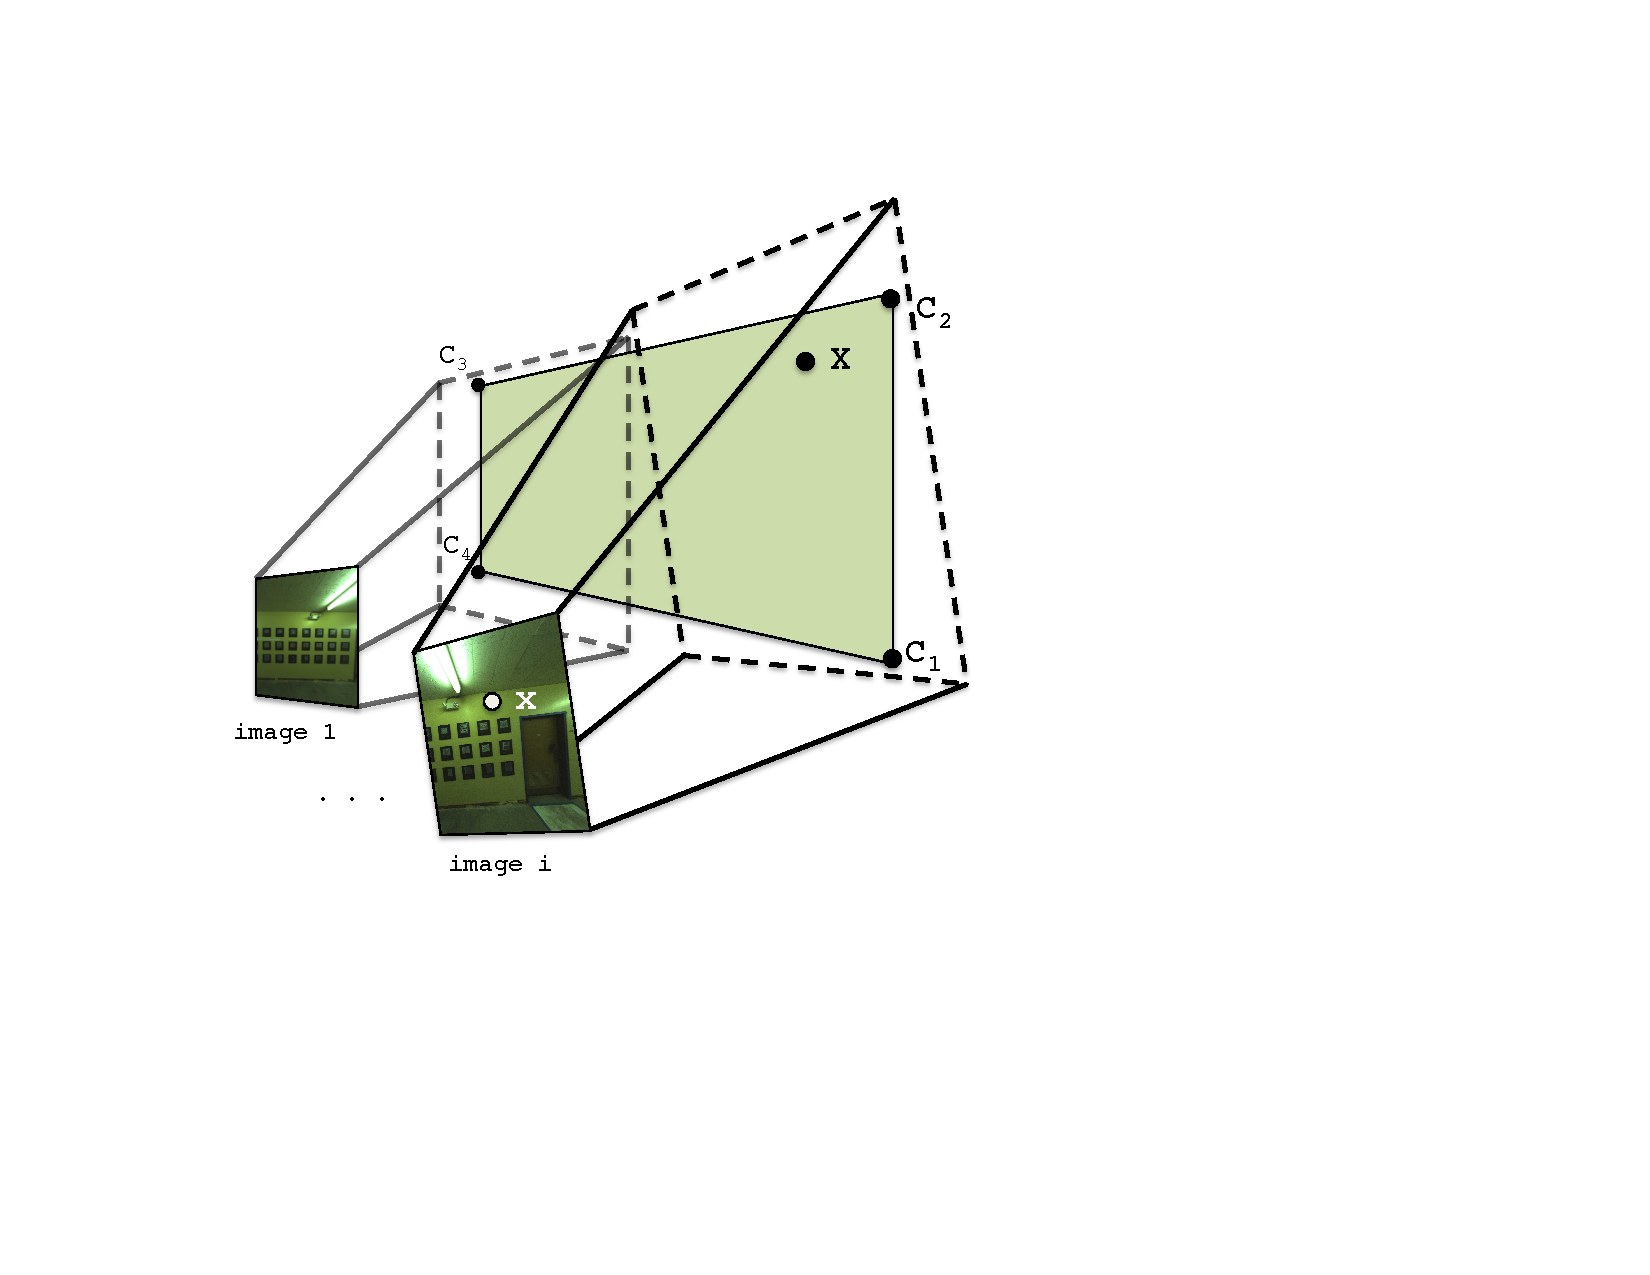
\includegraphics[height=2in]{Projection.pdf}
  \caption{Planes are specified in 3D space by four corners $C_1$ to
    $C_4$. Images are related to each plane through the camera
    matrices $P_{1..M}$. }
  % \caption{The plane is specified in 3D space by the four corners
  % $C_1$ to $C_4$. Images are related to the plane through the camera
  % matrices $P_{1..M}$. For example, the 3D point X in the world
  % coordinate system is related to the image point x shown in the
  % figure as $x = P_i X$.}
  \label{fig:projection}
\end{figure}

In this section, we will discuss the process of texture mapping a
single plane, as the texturing of each of our planes is completely
independent and can even be completed in parallel.  

The geometry of the general texture mapping process is shown in Figure 1. 

 As
described in the previous section, we are provided with a set of $M$
candidate images for each plane. Each image has a camera matrix $P_i$ for $i=1..M$, which
translates a 3D point in the world coordinate system to a 2D point in
image $i$'s coordinates. A camera matrix $P_i$ is composed of the
camera's intrinsic parameters, such as focal length and image center,
as well as the extrinsic parameters which specify the rotation and
translation of the camera center's position with respect to the world
coordinates at the time that image $i$ was taken. These extrinsic
parameters are determined by the localization hardware and algorithms
mentioned in Section \ref{sec:backpackSystem}. A point $X$ on the
plane in 3D space can be related to its corresponding pixel $x$ in image $i$
through the following equation:

\[
x=project(P_iX)
\]

where
\[X = \begin{pmatrix} x \\ y \\ z \end{pmatrix} \textrm{ and }
project(X) = \begin{pmatrix} x/z \\ y/z \end{pmatrix}
\]

A plane to be textured is defined by four corner vertices $C_1$ to $C_4$ in
world coordinates and a normal vector indicating the front facing side
of the plane. Our goal is to texture this plane using its associated
images, while eliminating any visual discontinuities or seams that
would suggest that the plane's texture was not composed of a single
continuous image.



\subsection{Naive Mapping}
\label{sec:naive}
\begin{figure}
  \centering
  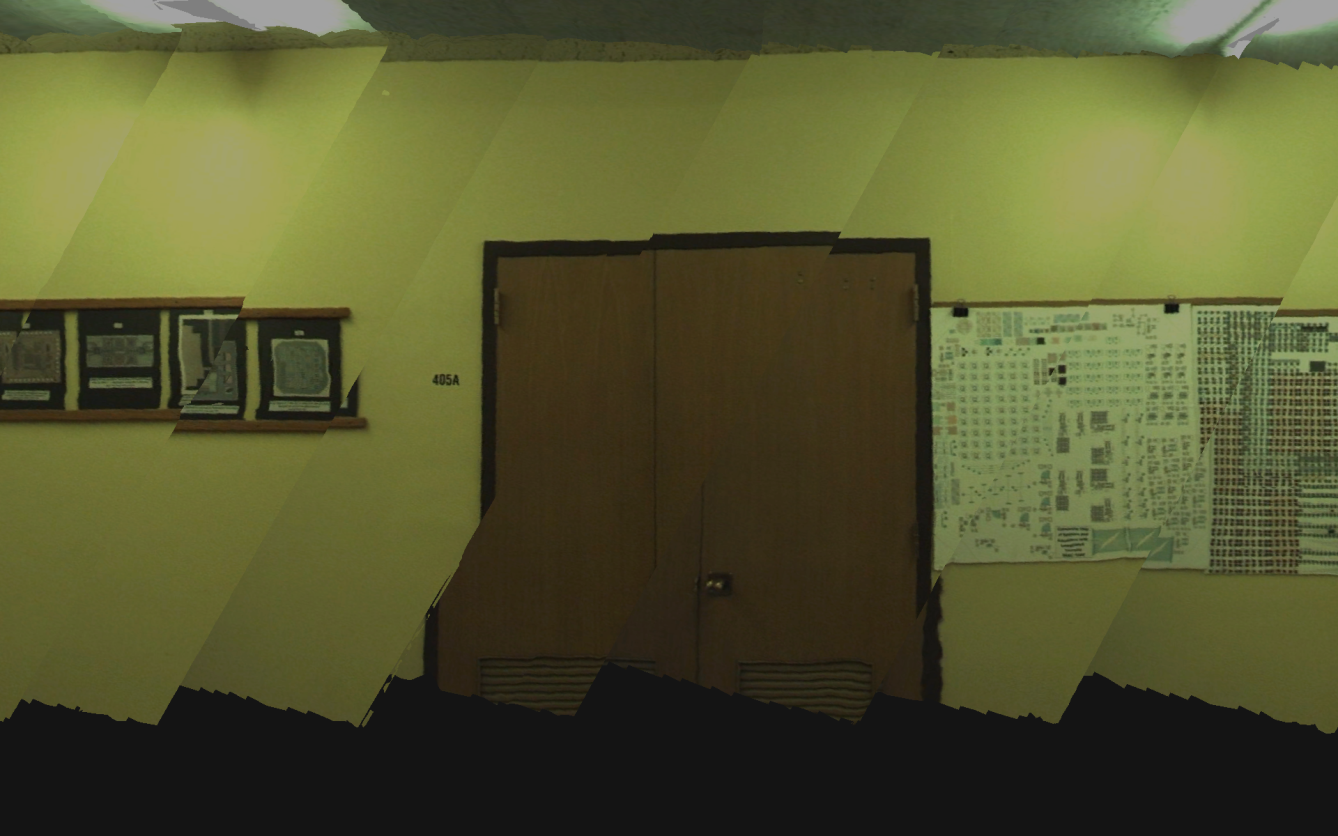
\includegraphics[height=1.5in]{naive.png}
  \caption{The result of naive texture mapping based on the imprecise
    camera matrices estimated by the localization system.}
  \label{fig:naive}
\end{figure}


Ignoring the fact that the camera matrices $P_{1..M}$ are inaccurate,
one can texture map the plane simply by discretizing the plane into
sections and texturing each section with one image. It makes sense to
texture each section by selecting the best image locally, as was done
in \ref{sec:imageAssociation}.

As Figure \ref{fig:naive} demonstrates, this naive mapping approach
leads to significant misalignment between successive tiles. This
suggests that while the errors in the localization system are quite
low, they are not pixel accurate. For photorealistic texture mapping,
either the camera matrices need to be refined such that the
localization is pixel accurate, resulting in a perfect mapping, or
image stitching techniques need to be applied to provide this
illusion. A commonly-used technique for each approach is examined
next.




\subsection{Image Mosaicing}

\begin{figure}
  \centering
  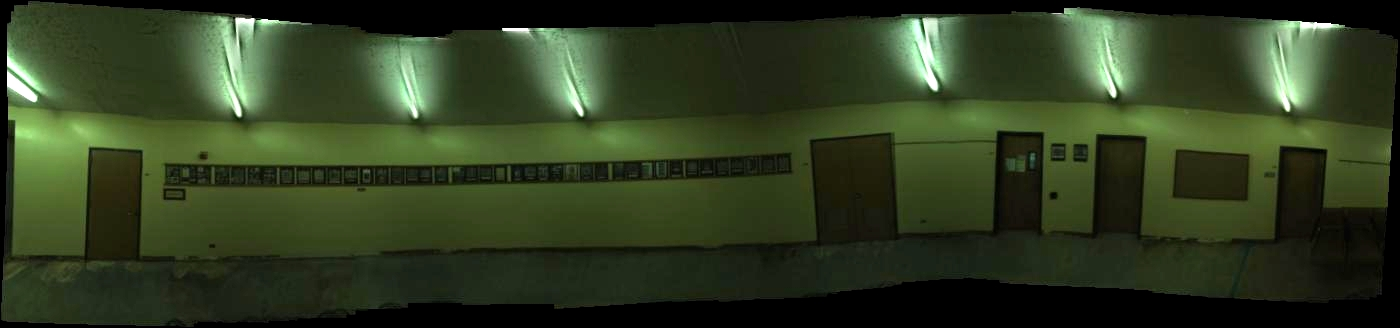
\includegraphics[width=3in]{panoMy.jpg}
  \caption{Image mosaicing. }
  \label{fig:mosaic}
\end{figure}


When images are taken of a plane from arbitrary overlapping positions,
they are related by homography \cite{hz}. Thus, existing
homography-based image mosaicing algorithms are applicable
\cite{brown2007automatic}. However, errors can compound when long
chains of images are mosaiced together using these approaches. For
example, a pixel in the $n$th image in the chain must be translated
into the first image's coordinates by multiplying by the $3\times3$
matrix $H_1 H_2 H_3 ... H_n$. Any error in one of these homography
matrices is propagated to all further images until the chain is
broken. For some chains of images this can happen almost immediately
due to erroneous correspondence matches and the resulting image mosaic
is grossly misshapen.

Figure \ref{fig:mosaic} shows the output of the AutoStitch software
package which does homography-based image mosaicing. This plane is
nearly a best-case scenerio with many features spread uniformly across
it. Even so, the mosaicing produces errors that causes straight lines
to appear as waves on the plane. This image was generated after
careful hand tuning. Many planes that had fewer features simply
failed. This led to the conclusion that image mosaicing is not a
robust enough solution for reliably texture mapping our dataset.

\subsection{Image-Based 3D Localization Refinement}

\begin{figure}
  \centering
  
\includegraphics[width=3in]{Graph_crop.pdf}
  \caption{Using the graph-based localization refinement algorithm
    from [11] suffers from the problem of compounding errors. }
  \label{fig:graph}
\end{figure}

Another approach is to refine the camera matrices using image
correspondences to guide the process. Each image's camera matrix has 6 degrees of freedom. Previous work has attempted to refine
camera matrices by solving a non-linear optimization problem
\cite{liu2010indoor}. This process is specific to the backpack system
which generated our dataset, as it must be run during backpack
localization\cite{liu2010indoor,chen2010indoor}. Unfortunately, this
approach suffers from a similar error propagation problem shown in
Figure \ref{fig:graph}. In our new approach, we also refine the
placement of images using image correspondences. However, we do so in
two dimensions on the plane whereas this previous work did so over all
6 degrees of freedom. Refining in two dimensions on the plane is less
flexible in that it does not address projection errors, however, it
provides noticeable benefits while avoiding the error propagation
problem.


\section{Our Approach Overview}
Our approach begins with the naive projection of all our images onto separate copies of our plane, such that no projected data is lost. We then perform a series of preprocessing steps to rotate and shift each image's projection such that its overlapping regions with other projections are as seamless as possible. Following this, we perform a basic intensity-matching algorithm across all images, as images taken from different locations have different levels of overall brightness. From here, we assign textures to our planes using one of two methods, dependent on whether they are wall planes or ceiling/floor planes. The reasoning for this is explained in section \ref{sec:whydifferent}. Lastly, we apply alpha blending to smooth out any remaining seams.

\subsection{Preprocessing}
As a starting point, we naively texture map the plane using the given imprecise camera matrices for each image in the set. This is done by discretizing the plane into an arbitrary density of pixels and projecting each pixel into the image plane using the estimated camera matrix $P_i$. We later intend to shift some of these projected images around on the plane and remove some others. Therefore, each image is stored intact in its own data structure so that it can later be merged with the other images on the plane. We use a Hough transform to rotate the projected images such that vertical lines are pointing directly upwards. This can be effective for indoor modeling, since many indoor scenes contain strong vertical lines from features such as doors, wall panels, or rectangular frames. 


\subsection{Localization Refinement}

The camera matrices generated by the localization algorithm are imprecise so the images are misaligned. To fix this, we choose to fix the locations in 2D. First we find corresponding points between all pairs of overlapping images using SIFT matches \cite{lowe1999object}. An illustration of this is given in Figure \ref{fig:matches}. The SIFT matches allow us to determine the correct $x$ and $y$ distances between two images on the plane. We already have an estimate of the $x$ and $y$ distances between the two images which was given by the localization algorithms. Soon we will compare the original estimates to the SIFT-based distances and use this to improve the quality of the image locations. 

\subsubsection{Robust SIFT Distances using RANSAC}

First we need to ensure that the SIFT-based distances are reliable. Since SIFT matches frequently include outliers, the RANSAC framework \cite{fischler1981random} is used for a robust estimate of the $x$ and $y$ distances between the two images. The RANSAC framework will attempt to build a consensus among the SIFT matches about what the true $x$ and $y$ distance is between the two images while ignoring the influence of outliers that may skew the results. The framework handles the consensus-building machinery, and only requires that two functions be specified: the fitting function and the distance function. These functions are called for random subsets of the SIFT matches until the best set of inliers is found. For this application, the fitting function simply finds the average distance between matches. If the matches are exactly correct and the image is frontal and planar then the distances for various SIFT feature matches should be the same. Our distance function for a pair of points is the difference between those points' SIFT match distance and the average distance computed by the fitting function. We specified a 10 pixel outlier threshold to the framework. This means that a SIFT match is labeled as an outlier if its $x$ and $y$ distance is not within 10 pixels of the average distance computed by the fitting function.

\subsubsection{Refining Image Positions using Least Squares}

There are a total of $M^{2}$ possible pairs of images, however we can only measure distances between images that overlap at SIFT feature points. Given these distances and the original image location estimates, we solve a least squares problem ($\textrm{min}_{\beta} ||\beta X - y||_2^2 $) to estimate the correct location of the images on the plane. The vector $\beta$ of unknowns are the correct $x$ and $y$ locations of each image on the plane from $1 \dots M$. Finding the correct $x$ and $y$ locations are independent from one another so we will only consider the $x$ locations:

% Draw least squares problem here. 

\[\beta =
 \begin{pmatrix}
  x_1, & x_2, & x_3, & \cdots & x_{M-1}, & x_M
 \end{pmatrix}
\]

The matrix $X$ is constructed with one row for each pair of images with measured distances produced by the SIFT matching stage. A row in the matrix has a $-1$ and $1$ in the columns corresponding to the two images in the pair. For example, the matrix below indicates that we generated a SIFT-based distance between images 1 and 2, images 1 and 3, images 2 and 3, etc. 

\[
 X =
 \begin{pmatrix}
  -1 & 1 & 0 & \cdots & 0 & 0\\
  -1 & 0 & 1 & \cdots & 0 & 0\\
   0 & -1 & 1 & \cdots & 0 & 0\\
  \vdots  & \vdots & \vdots & \ddots & \vdots  & \vdots\\
  0 & 0 & 0 & \cdots & 1 & 0 \\ 
  0 & 0 & 0 & \cdots & -1 & 1 \\ 
  1 & 0 & 0 & \cdots & 0 & 0 \\ 
 \end{pmatrix}
\]

If only relative distances between images are included then there is no way to determine the absolute location of any of the images and the matrix becomes rank deficient. To fix this we choose the first image to serve as the anchor for the rest, meaning all the absolute distances are based on its original location. This is done by adding a row with a $1$ in the first column and the rest zeros. 

Finally, the observation vector $y$ is constructed using the SIFT-based distances generated earlier in the matching stage. The distances are denoted as $d_1 \dots d_N$ for $N$ SIFT-based distances. The last element in the observation vector is the original location of the first image determined by the localization algorithm. 

\[
y^T = 
 \begin{pmatrix}
  d_{1,2}, & d_{1,3}, & d_{2,3}, & \hdots & d_{N-2,N-1}, & d_{N-1,N}, &  x_1
 \end{pmatrix}
\]

The $\beta$ that minimizes  $||\beta X - y||_2^2$ tells us a set of image locations on the plane that best honors all the SIFT-based distance measurements between images. A similar problem is solved for the $y$ dimension. In practice there are often cases where there is a break in the chain of images, meaning that no SIFT matches were found between one segment of the plane and another. In this case we add rows to the $X$ matrix and observations to the $y$ vector that contain the original $x$ and $y$ distance estimates generated by the localization algorithm. Another way to do this is to add rows for all neighboring pairs of images and solve a weighted least squares problem where the SIFT distances are given a higher weight i.e. 1, and the distances generated by the localization algorithm are given a smaller weight i.e. 0.01.

At this point we now have our target plane associated with a list of images as well as their rotated and shifted projections upon the plane. We are ready to begin assigning these projections to areas of our plane for texturing.



\subsection{Ceiling/Floor Texturing vs. Wall Texturing}
\label{sec:whydifferent}
The backpack
modeling system described in Section \ref{sec:backpackHardware} was designed to prioritize for
texturing walls. As mentioned previously, the backpack contains two
fisheye cameras, one aimed directly to the left of the backpack
operator, and one aimed directly to the right. Thus, in order to
texture the ceiling above where the operator walked, images from both
cameras must be combined, with their boundaries meeting overhead. Even more problematic, the floor beneath the
backpack is physically obscured by the operator's body, and thus must
be textured by images taken from behind the operator or from the side. This problem of distant cameras at poor angles
is compounded by the fact that the operator's data acquisition path
attempts to fully scan each wall, but not necessarily the entirety of
a floor or ceiling. This means that large swaths of floors and
ceilings are never walked directly over or under, and thus must be
textured by sidelong images taken from further distances and at
oblique angles. Images taken from closer distances are much preferred, as the effects of imprecise localization and camera matrices become multiplied over greater distances. We also strongly prefer head-on images because when images
are projected onto a planar surface at an extreme angle, the resultant
texture ends up spanning a large portion of the plane, applying
low-resolution textures to areas at greater distances from the camera
location.

In short, these factors mean that wall planes are generally associated with a
multitude of upright, uniform images, from a relatively close distance and originally taken head-on at regular intervals, while floors and
ceilings are associated with images taken from all manner of orientations and
distances. This major difference suggests we employ two strategies,
one tailored for each scenario.


\section{Texturing Walls}
Because wall images in general are all fairly good candidates for texturing due to their orientation and location, our goal is less about determining the best images to texture with individually, and more about selecting a set of images that together form the most seamless texture.

In order to objectively decide which sets of images form the most seamless textures, we need to decide on a cost function. We may be interested in covering the plane while minimizing the sum of squared pixel differences of the blended seam regions. This would encourage seams to be placed either in featureless areas, such as blank walls, or in areas in which the images are very well aligned. Another possible cost function is edge energy, i.e. the sum of the smoothed gradient of the blended seam regions. This would encourage seams to be placed in featureless areas even more than the sum of squared pixel difference cost function. For the dataset whose results are used in this paper, the first cost function is used, as the regular occurrence of featureless areas is not guaranteed.

\subsection{Image Selection}

Now that we have a cost function defined, we need to mechanically select the set of images for which the overall cost function is minimized.
By adding the constraint that we aim to cover the entirety of our plane, one could see how our problem generalizes to a graph coverage problem, as depicted in figure X. Returning again to the optimality of our situation when texturing walls however, we can make a quick simplification for the sake of efficiency. Given that our wall-texture candidate images were all taken from a head-on angle, we can reason that their projections onto the plane are approximately rectangular. By simply discarding any excess texture and cropping them all to be rectangular, our problem becomes the conceptually simpler problem of filling a polygon with rectangles, such that the sum of all edge costs between each pair of rectangles is minimal. 

maybe i dunno

Following the general scheme of Prim's algorithm for a minimum spanning tree, we can greedily add the minimal-cost image to our set until we have reached the desired coverage of our plane. This method can be applied on all manner of planes and images, howev this could be used for floors ceilings who knows



\begin{figure}
\centering
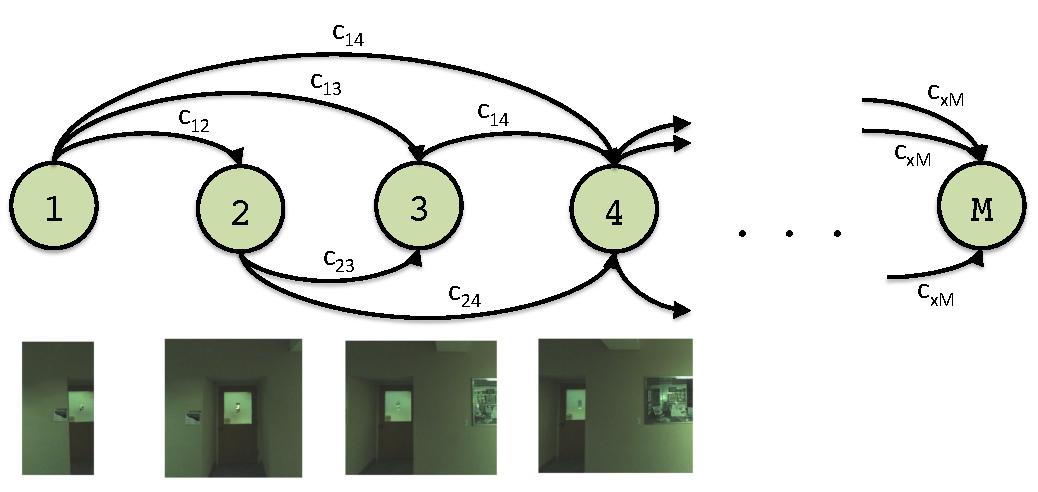
\includegraphics[width=3in]{DynProg.pdf}
\caption{Image Selection is done by constructing a graph of sorted images. Then we solve a shortest path problem where the edge weights represent the cost of a seam between two overlapping images.}
\label{fig:DynProg}
\end{figure}

By taking one more shortcut we can simplify our problem down even further. Since care is taken such that our wall images generally contain the floor-to-ceiling range of walls, we generally do not have any wall images such that one should be projected vertically above the other. In essence, we need only to ensure horizontal coverage of our planes, as our images generally line up together at the same height. We can thus construct a DAG from the images, again with edge costs defined by our cost function above, and solve a simple shortest path problem to find an optimal subset of images with regard to the cost functions.

Figure \ref{fig:DynProg} demonstrates the construction of a DAG from overlapping images of a long hallway. Images are sorted by location (e.g. left to right) and become nodes in a graph. Edges are placed in the graph between images that overlap. The weights of these edges are determined by a cost function, such as image energy, or the sum of squared pixel differences between the two images in the seam region. Next, we solve a shortest path problem from the first node in the graph to the last node. This provides a set of images that completely covers the plane, but minimizes the cost of the seams produced. Note that this only works when all the images completely cover one dimension. In this case the vertical dimension of the plane is covered by all images. 

In cases where the vertical dimension of the plane is not entirely covered, generally due to suboptimal camera locations, we are left with a hole where no image was chosen to texture. Rather than reverting to a 2D-coverage problem, we can elect to simply fill the hole by repeatedly selecting images in a greedy fashion, with respect to our cost function.

At this point, we have accounted for every location on our plane with an image or images that were selected. Before actually applying our textures, we will examine how to accomplish the same for ceilings and floors.

\subsection{Texturing Ceilings and Floors}


Because the images associated with ceilings and floors are often captured by cameras at sidelong angles, we must be conservative when texture mapping such planes. Since localization errors compound over distance, we often have candidate images that project well on areas near the camera itself, but much more poorly at greater distances. 

Furthermore, as a result of the projection process and cropping due to occlusion, The geometry of the usable texture projected onto the plane for each image is generally complex and difficult to work with.

These problems suggest that we must segment our images to some extent, as many of our images have desired as well as undesired portions. Such segmentation undoubtedly leads to more discontinuities, but floors and ceilings have lame textures


\subsection{Evaluation of Methods}
methods can be used on eachother







\section{NOTES}

\subsection{Occlusion Masking}
not sure where this section should go. it happens after projections,
discussed in texture mapping overview, but it's definitely more of a
preprocessing step.  Before we proceed with texturing our planes, we
need to ensure that each plane's associated images contain only
content that should be mapped onto the target plane in question. From
the above process, images were chosen such that they had an unoccluded
view of one or more trianglular sections upon a plane. This may not
necessarily hold true however for all areas of the plane, as
demonstrated in figure SOMETHING. If images are not modified to mask
out occluded areas, different images could attempt to cover the same
location on a plane with drastically different textures, inevitably
leading to undesireable discontinuities in our final texture.

Fortunately, by virtue of our indoor environments, the vast majority
of surface geometry is either horizontal or vertical, with high
amounts of right angles. This means that the areas we wish to mask out
of our images due to occlusion are nearly always rectangular
areas. Similar to the triangular tesselation performed for image
association above, we split our image into






With the steps in this section completed, we have generalized the
input of our texture mapping problem into rectangular planes that are
associated with a list of good candidate images, and we are ready to
begin the texture mapping process.






4.1 Texturing Floors and Ceilings




4.2 Texturing Walls Since our candidate images for texturing a wall
are all taken from similar distances and orientations relative to our
wall, their individual "qualities" are all fairly similar. We don't
have to worry as much about filtering out bad images; rather we seek
to select some subset of our images which together form a good
texture.

5 Results and Analysis but also occlusion projection thing. door
projected onto wall is fine, door projected onto floor is bad.

\section{EVERYTHING AFTER HERE IS TEMPLATE STUFF}






\section{Introduction}

Please follow the steps outlined below when submitting your manuscript
to the IEEE Computer Society Press.  This style guide now has several
important modifications (for example, you are no longer warned against
the use of sticky tape to attach your artwork to the paper), so all
authors should read this new version.

% -------------------------------------------------------------------------
\subsection{Language}

All manuscripts must be in English.

\subsection{Dual submission}

By submitting a manuscript to 3DIMPVT, the authors assert that it has
not been previously published in substantially similar
form. Furthermore, no paper which contains significant overlap with
the contributions of this paper either has been or will be submitted
during the 3DIMPVT 2012 review period to {\bf either a journal} or any
conference or any workshop.  {\bf Papers violating this condition will
  be rejected}.

If there are papers that may appear to the reviewers to violate this
condition, then it is your responsibility to: (1)~cite these papers
(preserving anonymity as described in Section 1.6 below), (2)~argue in
the body of your paper why your 3DIMPVT paper is non-trivially
different from these concurrent submissions, and (3)~include
anonymized versions of those papers in the supplemental material.

\subsection{Paper length}
3DIMPVT papers may be between 6 pages and 8 pages.  Overlength papers
will simply not be reviewed.  This includes papers where the margins
and formatting are deemed to have been significantly altered from
those laid down by this style guide.  Note that this \LaTeX\ guide
already sets figure captions and references in a smaller font.  The
reason such papers will not be reviewed is that there is no provision
for supervised revisions of manuscripts.  The reviewing process cannot
determine the suitability of the paper for presentation in eight pages
if it is reviewed in eleven.

% -------------------------------------------------------------------------
\subsection{The ruler}
The \LaTeX\ style defines a printed ruler which should be present in
the version submitted for review.  The ruler is provided in order that
reviewers may comment on particular lines in the paper without
circumlocution.  If you are preparing a document using a non-\LaTeX\
document preparation system, please arrange for an equivalent ruler to
appear on the final output pages.  The presence or absence of the
ruler should not change the appearance of any other content on the
page.  The camera ready copy should not contain a ruler. (\LaTeX\
users may uncomment the \verb'\cvprfinalcopy' command in the document
preamble.)  Reviewers: note that the ruler measurements do not align
well with lines in the paper --- this turns out to be very difficult
to do well when the paper contains many figures and equations, and,
when done, looks ugly.  Just use fractional references (e.g.\ this
line is $097.15$), although in most cases one would expect that the
approximate location will be adequate.

\subsection{Mathematics}

Please number all of your sections and displayed equations.  It is
important for readers to be able to refer to any particular equation.
Just because you didn't refer to it in the text doesn't mean some
future reader might not need to refer to it.  It is cumbersome to have
to use circumlocutions like ``the equation second from the top of page
3 column 1''.  (Note that the ruler will not be present in the final
copy, so is not an alternative to equation numbers).  All authors will
benefit from reading Mermin's description of how to write mathematics:
\url{http://www.cvpr.org/doc/mermin.pdf}.


\subsection{Blind review}

Many authors misunderstand the concept of anonymizing for blind
review.  Blind review does not mean that one must remove citations to
one's own work---in fact it is often impossible to review a paper
unless the previous citations are known and available.

Blind review means that you do not use the words ``my'' or ``our''
when citing previous work.  That is all.  (But see below for
techreports)

Saying ``this builds on the work of Lucy Smith [1]'' does not say that
you are Lucy Smith, it says that you are building on her work.  If you
are Smith and Jones, do not say ``as we show in [7]'', say ``as Smith
and Jones show in [7]'' and at the end of the paper, include reference
7 as you would any other cited work.

An example of a bad paper just asking to be rejected:
\begin{quote}
  \begin{center}
    An analysis of the frobnicatable foo filter.
  \end{center}

  In this paper we present a performance analysis of our previous
  paper [1], and show it to be inferior to all previously known
  methods.  Why the previous paper was accepted without this analysis
  is beyond me.

  [1] Removed for blind review
\end{quote}


An example of an acceptable paper:

\begin{quote}
  \begin{center}
    An analysis of the frobnicatable foo filter.
  \end{center}

  In this paper we present a performance analysis of the paper of
  Smith \etal [1], and show it to be inferior to all previously known
  methods.  Why the previous paper was accepted without this analysis
  is beyond me.

  [1] Smith, L and Jones, C. ``The frobnicatable foo filter, a
  fundamental contribution to human knowledge''.  Nature 381(12),
  1-213.
\end{quote}

If you are making a submission to another conference at the same time,
which covers similar or overlapping material, you may need to refer to
that submission in order to explain the differences, just as you would
if you had previously published related work.  In such cases, include
the anonymized parallel submission~\cite{Authors12} as additional
material and cite it as
\begin{quote} [1] Authors. ``The frobnicatable foo filter'', F\&G 2012
  Submission ID 324, Supplied as additional material {\tt fg324.pdf}.
\end{quote}

Finally, you may feel you need to tell the reader that more details
can be found elsewhere, and refer them to a technical report.  For
conference submissions, the paper must stand on its own, and not {\em
  require} the reviewer to go to a techreport for further details.
Thus, you may say in the body of the paper ``further details may be
found in~\cite{Authors12b}''.  Then submit the techreport as
additional material.  Again, you may not assume the reviewers will
read this material.

Sometimes your paper is about a problem which you tested using a tool
which is widely known to be restricted to a single institution.  For
example, let's say it's 1969, you have solved a key problem on the
Apollo lander, and you believe that the CVPR70 audience would like to
hear about your solution.  The work is a development of your
celebrated 1968 paper entitled ``Zero-g frobnication: How being the
only people in the world with access to the Apollo lander source code
makes us a wow at parties'', by Zeus \etal.

You can handle this paper like any other.  Don't write ``We show how
to improve our previous work [Anonymous, 1968].  This time we tested
the algorithm on a lunar lander [name of lander removed for blind
review]''.  That would be silly, and would immediately identify the
authors. Instead write the following:
\begin{quotation}
  \noindent
  We describe a system for zero-g frobnication.  This system is new
  because it handles the following cases: A, B.  Previous systems
  [Zeus et al. 1968] didn't handle case B properly.  Ours handles it
  by including a foo term in the bar integral.

  ...

  The proposed system was integrated with the Apollo lunar lander, and
  went all the way to the moon, don't you know.  It displayed the
  following behaviours which show how well we solved cases A and B:
  ...
\end{quotation}
As you can see, the above text follows standard scientific convention,
reads better than the first version, and does not explicitly name you
as the authors.  A reviewer might think it likely that the new paper
was written by Zeus \etal, but cannot make any decision based on that
guess.  He or she would have to be sure that no other authors could
have been contracted to solve problem B.

FAQ: Are acknowledgements OK?  No.  Leave them for the final copy.


\begin{figure}[t]
  \begin{center}
    \fbox{\rule{0pt}{2in} \rule{0.9\linewidth}{0pt}}
    % \includegraphics[width=0.8\linewidth]{egfigure.eps}
  \end{center}
  \caption{Example of caption.  It is set in Roman so that mathematics
    (always set in Roman: $B \sin A = A \sin B$) may be included
    without an ugly clash.}
  \label{fig:long}
  \label{fig:onecol}
\end{figure}

\subsection{Miscellaneous}

\noindent
Compare the following:\\
\begin{tabular}{ll}
  \verb'$conf_a$' &  $conf_a$ \\
  \verb'$\mathit{conf}_a$' & $\mathit{conf}_a$
\end{tabular}\\
See The \TeX book, p165.

The space after \eg, meaning ``for example'', should not be a
sentence-ending space. So \eg is correct, {\em e.g.} is not.  The
provided \verb'\eg' macro takes care of this.

When citing a multi-author paper, you may save space by using ``et
alia'', shortened to ``\etal'' (not ``{\em et.\ al.}'' as ``{\em et}''
is a complete word.)  However, use it only when there are three or
more authors.  Thus, the following is correct: `` Frobnication has
been trendy lately.  It was introduced by Alpher~\cite{Alpher02}, and
subsequently developed by Alpher and
Fotheringham-Smythe~\cite{Alpher03}, and Alpher
\etal~\cite{Alpher04}.''

This is incorrect: ``... subsequently developed by Alpher
\etal~\cite{Alpher03} ...''  because reference~\cite{Alpher03} has
just two authors.  If you use the \verb'\etal' macro provided, then
you need not worry about double periods when used at the end of a
sentence as in Alpher \etal.

For this citation style, keep multiple citations in numerical (not
chronological) order, so prefer \cite{Alpher03,Alpher02,Authors12} to
\cite{Alpher02,Alpher03,Authors12}.


\begin{figure*}
  \begin{center}
    \fbox{\rule{0pt}{2in} \rule{.9\linewidth}{0pt}}
  \end{center}
  \caption{Example of a short caption, which should be centered.}
  \label{fig:short}
\end{figure*}

% ------------------------------------------------------------------------
\section{Formatting your paper}

All text must be in a two-column format. The total allowable width of
the text area is $6\frac78$ inches (17.5 cm) wide by $8\frac78$ inches
(22.54 cm) high. Columns are to be $3\frac14$ inches (8.25 cm) wide,
with a $\frac{5}{16}$ inch (0.8 cm) space between them. The main title
(on the first page) should begin 1.0 inch (2.54 cm) from the top edge
of the page. The second and following pages should begin 1.0 inch
(2.54 cm) from the top edge. On all pages, the bottom margin should be
1-1/8 inches (2.86 cm) from the bottom edge of the page for $8.5
\times 11$-inch paper; for A4 paper, approximately 1-5/8 inches (4.13
cm) from the bottom edge of the page.

% -------------------------------------------------------------------------
\subsection{Margins and page numbering}

All printed material, including text, illustrations, and charts, must
be kept within a print area 6-7/8 inches (17.5 cm) wide by 8-7/8
inches (22.54 cm) high.


% -------------------------------------------------------------------------
\subsection{Type-style and fonts}

Wherever Times is specified, Times Roman may also be used. If neither
is available on your word processor, please use the font closest in
appearance to Times to which you have access.

MAIN TITLE. Center the title 1-3/8 inches (3.49 cm) from the top edge
of the first page. The title should be in Times 14-point, boldface
type.  Capitalize the first letter of nouns, pronouns, verbs,
adjectives, and adverbs; do not capitalize articles, coordinate
conjunctions, or prepositions (unless the title begins with such a
word). Leave two blank lines after the title.

AUTHOR NAME(s) and AFFILIATION(s) are to be centered beneath the title
and printed in Times 12-point, non-boldface type. This information is
to be followed by two blank lines.

The ABSTRACT and MAIN TEXT are to be in a two-column format.

MAIN TEXT. Type main text in 10-point Times, single-spaced. Do NOT use
double-spacing. All paragraphs should be indented 1 pica (approx. 1/6
inch or 0.422 cm). Make sure your text is fully justified---that is,
flush left and flush right. Please do not place any additional blank
lines between paragraphs.

Figure and table captions should be 9-point Roman type as in
Figures~\ref{fig:onecol} and~\ref{fig:short}.  Short captions should
be centred.

\noindent Callouts should be 9-point Helvetica, non-boldface type.
Initially capitalize only the first word of section titles and first-,
second-, and third-order headings.

FIRST-ORDER HEADINGS. (For example, {\large \bf 1. Introduction})
should be Times 12-point boldface, initially capitalized, flush left,
with one blank line before, and one blank line after.

SECOND-ORDER HEADINGS. (For example, { \bf 1.1. Database elements})
should be Times 11-point boldface, initially capitalized, flush left,
with one blank line before, and one after. If you require a
third-order heading (we discourage it), use 10-point Times, boldface,
initially capitalized, flush left, preceded by one blank line,
followed by a period and your text on the same line.

% -------------------------------------------------------------------------
\subsection{Footnotes}

Please use footnotes\footnote {This is what a footnote looks like.  It
  often distracts the reader from the main flow of the argument.}
sparingly.  Indeed, try to avoid footnotes altogether and include
necessary peripheral observations in the text (within parentheses, if
you prefer, as in this sentence).  If you wish to use a footnote,
place it at the bottom of the column on the page on which it is
referenced. Use Times 8-point type, single-spaced.


% -------------------------------------------------------------------------
\subsection{References}

List and number all bibliographical references in 9-point Times,
single-spaced, at the end of your paper. When referenced in the text,
enclose the citation number in square brackets, for
example~\cite{Authors12}.  Where appropriate, include the name(s) of
editors of referenced books.

\begin{table}
  \begin{center}
    \begin{tabular}{|l|c|}
      \hline
      Method & Frobnability \\
      \hline\hline
      Theirs & Frumpy \\
      Yours & Frobbly \\
      Ours & Makes one's heart Frob\\
      \hline
    \end{tabular}
  \end{center}
  \caption{Results.   Ours is better.}
\end{table}

% -------------------------------------------------------------------------
\subsection{Illustrations, graphs, and photographs}

All graphics should be centered.  Please ensure that any point you
wish to make is resolvable in a printed copy of the paper.  Resize
fonts in figures to match the font in the body text, and choose line
widths which render effectively in print.  Many readers (and
reviewers), even of an electronic copy, will choose to print your
paper in order to read it.  You cannot insist that they do otherwise,
and therefore must not assume that they can zoom in to see tiny
details on a graphic.

When placing figures in \LaTeX, it's almost always best to use
\verb+\includegraphics+, and to specify the figure width as a multiple
of the line width as in the example below {\small\begin{verbatim}
    \usepackage[dvips]{graphicx} ...
   \includegraphics[width=0.8\linewidth]
                   {myfile.eps}
\end{verbatim}
}


% -------------------------------------------------------------------------
\subsection{Color}

Color is valuable, and will be visible to readers of the electronic
copy.  However ensure that, when printed on a monochrome printer, no
important information is lost by the conversion to grayscale.

% ------------------------------------------------------------------------
\section{Final copy}

You must include your signed IEEE copyright release form when you
submit your finished paper. We MUST have this form before your paper
can be published in the proceedings.

% Please direct any questions to the production editor in charge of
% these proceedings at the IEEE Computer Society Press: Phone (714)
% 821-8380, or Fax (714) 761-1784.

{\small \bibliographystyle{ieee} \bibliography{egbib} }


\end{document}
